\documentclass[conference]{IEEEtran}
\IEEEoverridecommandlockouts
% The preceding line is only needed to identify funding in the first footnote. If that is unneeded, please comment it out.
\usepackage{cite}
\usepackage{amsmath,amssymb,amsfonts}
\usepackage{algorithmic}
\usepackage{graphicx}
\usepackage{textcomp}
\usepackage[table,xcdraw]{xcolor}
\usepackage{longtable}
\usepackage{graphicx}
\usepackage{placeins}
\usepackage{ragged2e}
\graphicspath{{resources/}}
\def\BibTeX{{\rm B\kern-.05em{\sc i\kern-.025em b}\kern-.08em
    T\kern-.1667em\lower.7ex\hbox{E}\kern-.125emX}}

\makeatletter
\let\oldlt\longtable
\let\endoldlt\endlongtable
\def\longtable{\@ifnextchar[\longtable@i \longtable@ii}
\def\longtable@i[#1]{\begin{figure}[t]
\onecolumn
\begin{minipage}{0.5\textwidth}
\oldlt[#1]
}
\def\longtable@ii{\begin{figure}[t]
\onecolumn
\begin{minipage}{0.5\textwidth}
\oldlt
}
\def\endlongtable{\endoldlt
\end{minipage}
\twocolumn
\end{figure}}
\makeatother
    


\begin{document}

\title{Interaction Design of Google Digital Wellbeing Application using User-Centered Design Approach}

\author{
  \IEEEauthorblockN{Gregorius Jovan Kresnadi}
  \IEEEauthorblockA{\textit{School of Electrical Engineering and Informatics} \\
    Institut Teknologi Bandung\\
    Bandung, Indonesia \\
    kresnadi30@gmail.com}
  \and
  \IEEEauthorblockN{Adi Mulyanto, S.T, M.T.}
  \IEEEauthorblockA{\textit{School of Electrical Engineering and Informatics} \\
    Institut Teknologi Bandung\\
    Bandung, Indonesia \\
    adi@informatika.org}
}

\maketitle

\begin{abstract}
  % $ latar belakang
  The increasing use of smartphones is negatively affecting the digital well-being of its users. Excessive use of smartphone can lead users to have high dependency to the point of addiction. This case raises the urgency for research in the field of Human Computer Interaction on the intentionality of not using technology. This research led to the concept of Digital Wellbeing, which Google has adopted to develop an app with such concept. However, it was found that the app had several problems according to complaints in the app reviews regarding the lack of utility provided.

  % $ proses penelitian
  Therefore, it is necessary to develop the interaction design for an application that can overcome the problems of the Google Digital Wellbeing application. The design process uses the User-Centered Design methodology. Data collection begins with analyzing reviews of the Digital Wellbeing application, then completed with interviews with application users. The result of the final project is a high-fidelity prototype of the application for Android mobile device display. The interaction design is designed by prioritizing usability goals of utility and learnability, and directing to user experience goals of helpful and motivating.

  % $ hasil penelitian
  Usability testing is done with targeted users in accordance with the specified personas, using measurement metrics such as SUS, SEQ, and IMI with Value/Usefulness, Interest/Enjoyment, and Pressure/Tension subscales to measure the achievement of goals. The test results showed that the prototype successfully solved the problems found and achieved the expected goals. It was concluded that the Search bar, App Group, and Activation Schedule features of the prototype play a major role in improving the utility of the application, and the Daily Goal feature is a leading feature in increasing user motivation to improve their digital habits.
  
\end{abstract}

\vspace{0.2cm}

\begin{IEEEkeywords}
  \textit{Digital Wellbeing, interaction design, user-centered design, prototype, widget}
\end{IEEEkeywords}

\section{Introduction}

Technology and the internet are essential necessities in human life in the 21st century. One of the most useful forms of modern technology that is easily accessible to humans is the smartphone, which includes internet access. Based on research collected on bankmycell.com, in 2021 there were 6.37 billion smartphone users in the world or around 80.68\% of the world's population, of which 160.23 million are residents of Indonesia \cite{turner2022howmanysmartphones}.

A lot of work can be done using various types of applications in a smartphone. According to research conducted by BusinessofApps, the number of apps on the iOS App Store when it was first launched in 2008 was 500, in November 2021 that number jumped to 1.85 million apps \cite{businessofapps2021}. Android users have even more options with a total of 2.56 million apps on the Google Play Store. With so many apps, by 2020 smartphone users have downloaded 142.9 billion apps, of which 56.1 billion downloads were for mobile games.

Emerging technology can improve the digital wellbeing of its users, in ways such as enhancing social connections, supporting mental health, and supporting healthy habits with flexibility in work practices. However, technology can also have adverse effects that lead to unhealthy patterns of its use. Some examples of adverse effects are loss of focus, fear of missing out (FoMO), and digital addiction. These bad traits can appear more often when time spent in the virtual world is not balanced with time in the real world \cite{ALMOURAD2021101778}.

Addictive behavior on smartphones have brought attention to researchers in the field of Human Computer Interaction (HCI) to conduct studies on the intentionality of not using technology. The study gave rise to the concept of "Digital Wellbeing" which focuses on improving user well-being in the use of digital media \cite{unesco2015dwconference}. Currently, there are many software on smartphones that apply this concept to change user behavior, one of which is made by Google \cite{CHI2019SOCIALIZE}. To help its users, Google released an application with the same name, Digital Wellbeing, so that users can utilize technology to improve their quality of life rather than being a distraction. On its website about Digital Wellbeing, Google said: "We're committed to giving everyone the tools they need to develop their own sense of digital wellbeing. So that life, not the technology in it, stays front and center" \cite{google2019digitalwellbeing}. 

\section{Literature Review}
% \subsection{Smartphone Addiction}
% According to research on the Smartphone Addiction Scale by Kwon et al, although smartphone addiction is not yet listed as the behavioral addiction in the DSM-5 (Diagnostic and Statistical Manual of Mental Disorders), addiction to activities that can be performed on the internet through smartphones, such as playing games, chatting, and pornography, show the same level of addiction as victims of drug and alcohol addiction \cite{10.1371/journal.pone.0083558}.

% A research by Roffarello dan De Russis found that excessive smartphone use has a negative effect on mental health and social interaction \cite{CHI2019SOCIALIZE}. This can be seen in the quality of in-person peer interaction, which usually requires effort and commitment to establish a good relationship, being affected by the concept of indirect interaction through smartphones where relationships are more diffuse with less interaction. Smartphones also often act as a source of distraction that diverts attention from important activities. These distractions can come from external stimuli such as smartphone notifications, but can also come from internal stimuli such as the urge to check email or play games. Users who experience these regular and unpredictable internal and external distractions tend to feel unproductive and stressed more often.

\subsection{Digital Wellbeing}
In response to the problem of smartphone overuse, researchers in the field of HCI began to aggressively study the intentionality of not using technology. In response, researchers, companies, and organizations worldwide came up with the term Digital Wellbeing to express the health of the relationship between users and their technology. According to the Forum for Well-being in Digital Media under UNESCO, Digital Wellbeing is the improvement of user well-being in the use of digital media. Wellbeing is a person's valuable psychological asset for survival and ongoing positive experiences \cite{unesco2015dwconference}.

In May 2018 at the Google I/O conference, Google launched Digital Wellbeing, a design philosophy that will be used in its products that aims to provide a better relationship between users and the technology they use. It is explained that Digital Wellbeing is about creating a healthy relationship with technology and keeping that relationship healthy. Google realizes that rapidly developing technology has become a challenge in maintaining a balance of time spent between the real world and the virtual world. Therefore, the concept of Digital Wellbeing presented by Google invites users to take control of technology so that it can provide the maximum possible benefits and potential and help achieve goals, rather than being a nuisance, distraction, or obstacle \cite{google2019dwcourse}.

Digital Wellbeing provides 6 design principles that can guide a design towards creating a healthier relationship with its users \cite{google2021dwframework}:

\begin{enumerate}
  \item Empowerment; thoughtful default settings can help people use tech in balanced, intentional ways. Therefore it is good practice to have supportive default settings on designs.

  \item Awareness; people are more likely to make positive choices when they notice what they are doing. A supportive design should illuminate behavior data and help people set goals.

  \item Control; By providing transparency towards settings, designs can anticipate users with diverse needs, abilities, and backgrounds. Providing in-depth settings can help many users achieve their specific goals. This should also be supported by clear explanations and transparency about how things work.

  \item Adaptability; it is important to consider the ability of features to adapt to different user contexts. Integrating the app experience with the user's context such as time, location, or the device being used can reduce the user's navigational cost.

\end{enumerate}

Google Digital Wellbeing is a distraction-prevention app that was launched alongside the design philosophy, available within the Android OS since version 9.0 (Android Pie) \cite{google2021dwsupport}. The app acts as a tool to help optimize the use of smartphones, designed to help users coexist with digital technology that always attracts attention and takes up time \cite{8976353}. The app consists of several key features:

\begin{enumerate}
  \item Dashboard; a control center to monitor the user's smartphone usage. Usage data consists of time spent on an app, unlock count, and notifications received. 
  \item App Timer; a way to limit the daily usage of an app. If the user exceeds the time limit, then the app will be blocked for the rest of the day.
  \item Focus Mode; lets users select distracting apps and pause them temporarily. Users can also set a schedule to automatically turn Focus Mode on.
  \item Bedtime Mode; quites the user's phone for better sleep. Can be scheduled to run automatically when bedtime, turning the screen to grayscale and silencing notifications with Do Not Disturb.
\end{enumerate}

\subsection{Interaction Design}

Interaction design is the process of designing an interactive product to create an experience that improves the quality of the workings, communication, and interaction of the product's users. Interaction design can also be seen as a fundamental basis in several disciplines, fields, and approaches related to the research and design process of computer-based systems. Therefore, it is often the case that some aspects of approaches that use interaction design guidelines often overlap \cite{PreeceRogersSharp15}. There are 4 approaches to designing interaction \cite{saffer2010designing}:

\begin{enumerate}
  \item User-Centered Design (UCD); focuses on designing around the user. Designers are responsible for understanding user needs and goals, and involving users throughout the design process.
  \item Activity-Centered Design (ACD); focuses on designing around the activities that users perform from start to finish. Designers are responsible for collecting behavior data and formulate it into a product design.
  \item Systems Design; focuses on the system as a whole, consisting of components such as the users, hardware, software, and other objects. Users play a part to set goals, while the design still revolves around the system.
  \item Genius Design; relies heavily on the designer's knowledge and creativity. Users provide validation for the design, without getting involved in the process.
\end{enumerate}

% If these approaches are compared using the designer's role and user's involvement as parameters, then the comparison can be summarized as explained in Table \ref{tab:design_approaches}.

% \RaggedLeft
% \begin{table}[htbp]
%   \caption{Approaches in Interaction Design \cite{saffer2010designing}}
%   \begin{footnotesize}
%     \begin{center}
%       \begin{tabular}{|m{0.12\linewidth}|m{0.22\linewidth}|m{0.22\linewidth}|m{0.22\linewidth}|}
%         \hline
%       \textbf{Approach} & \textbf{Overview} & \textbf{Users} & \textbf{Designer}\\ \hline
%       User-Centered Design & Focus on user needs and goals & The guides of design & Translator of user needs and goals\\ \hline
%       Activity-Centered Design & Focus on the tasks and activities that need to be accomplished & Performers of the activities & Creates tools for actions \\ \hline
%       Systems Design & Focus on the components of a system & Set the goals of the system & Makes sure all the parts of the system are in place \\ \hline
%       Genius Design & Skill and wisdom of designers used to make products & Source of validation & The source of inspiration \\ \hline
%     \end{tabular}
%     \label{tab:design_approaches}
%   \end{center}
% \end{footnotesize}
% \end{table}
% \justifying

% \RaggedLeft
% \begin{scriptsize}
% \begin{longtable}[c]{|m{0.15\linewidth}|m{0.25\linewidth}|m{0.25\linewidth}|m{0.25\linewidth}|}
%   \caption{Approaches in Interaction Design \cite{saffer2010designing}}
%   \label{tab:design_approaches} \\
%   \hline \rowcolor[HTML]{A3E5F5}
%   \centering\textbf{Approach} & \centering\textbf{Overview} & \textbf{Users} & \textbf{Designer} \\ \hline \endfirsthead
%   \hline \rowcolor[HTML]{A3E5F5}
%   \centering\textbf{Approach} & \centering\textbf{Overview} & \textbf{Users} & \textbf{Designer} \\ \hline \endhead

%   \hline \endfoot

%   User-Centered Design & Focus on user needs and goals & The guides of design & Translator of user needs and goals\\ \hline
%   Activity-Centered Design & Focus on the tasks and activities that need to be accomplished & Performers of the activities & Creates tools for actions \\ \hline
%   Systems Design & Focus on the components of a system & Set the goals of the system & Makes sure all the parts of the system are in place \\ \hline
%   Genius Design & Skill and wisdom of designers used to make products & Source of validation & The source of inspiration \\ \hline

% \end{longtable}
% \end{scriptsize}
% \justifying
% \FloatBarrier

\section{User Research and Analysis}

% In this research, User-Centered Design is chosen as the prefered approach for designing the interaction. The process follows the ISO 9241-210:2010 guideline \cite{iso9241-210:2010}, with detailed steps as follows. The process begins with determining the scope of development, then followed by understanding user characteristics, goals, and behaviors related to the problems. Next, the design solution is developed in the form of prototypes. The prototypes are then evaluated with usability testing where it is determined if the current solution is enough or needs further development. The whole process is done iteratively, in which the iteration can be done multiple times until the design solution meets the user requirements. Figure \ref{fig:ucd} illustrates the overall UCD process.

In this research, User-Centered Design is chosen as the prefered approach for designing the interaction. The process follows the ISO 9241-210:2010 guideline \cite{iso9241-210:2010}, illustrated in Figure \ref{fig:ucd}.

\begin{figure}[htbp]
  \centerline{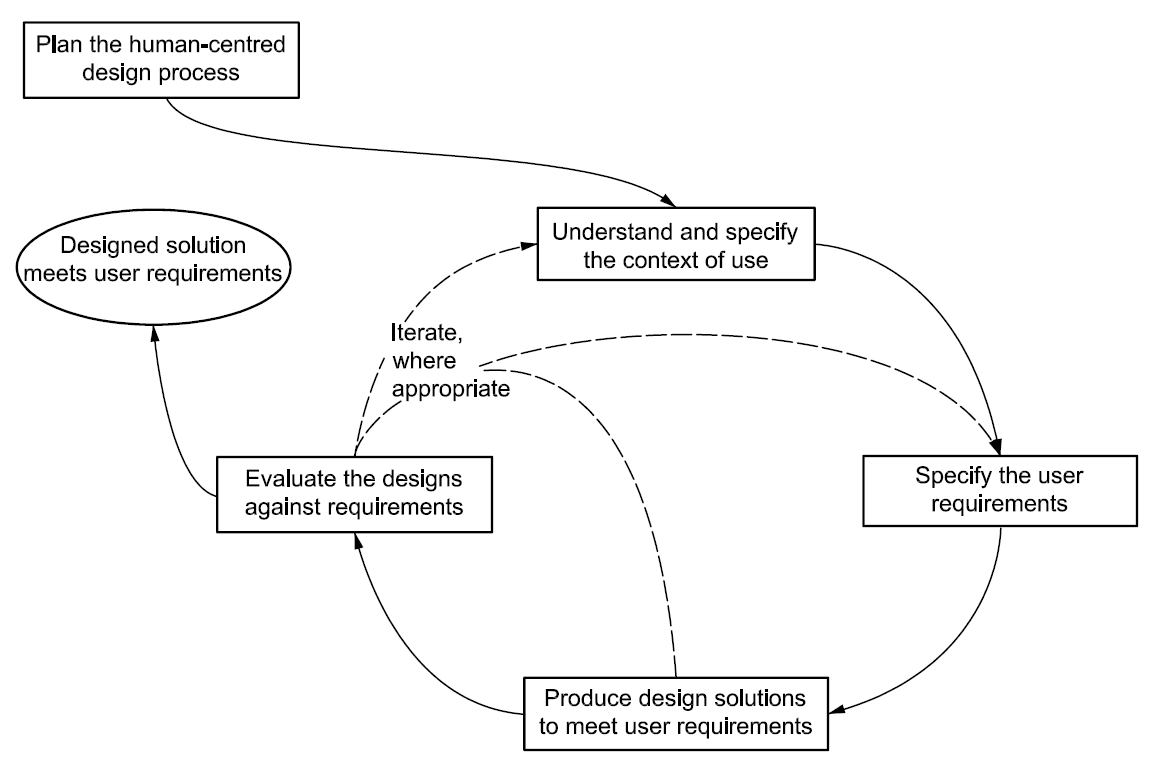
\includegraphics[width=0.9\linewidth]{ucd-figure.png}}
  \caption{User-Centered Design \cite{iso9241-210:2010}} \label{fig:ucd}
\end{figure}

\subsection{Specifying the Context of Use}

The target users of the research are Android-based smartphone users in Indonesia with an age range of 18-34 years. According to a research by Statista, it is the age range of the majority of social media users in Indonesia \cite{mediasosial2020}.

After the scope is determined, most recent user reviews of the Digital Wellbeing app are analyzed to understand the overall problem. This is done in accordance to the ISO guideline that available data of a product may be used to improve the quality of the product \cite{iso9241-210:2010}. User reviews are then categorized, as seen in Table \ref{tab:reviews}. Code "C" stands for Category.

\RaggedLeft
\begin{table}[htbp]
  \caption{User Review Categories of Google Digital Wellbeing}
  \begin{footnotesize}
    \begin{center}
      \begin{tabular}{|m{0.07\linewidth}|m{0.8\linewidth}|}
        \hline
        \centering\textbf{ID} & \textbf{Review Category}\\ \hline
      \centering C-01    & Lack of widgets that contain key features \\ \hline
      \centering C-02    & Lack of utility in the Dashboard page \\ \hline
      \centering C-03    & Focus Mode needs more strictness \\ \hline
      \centering C-04    & Lack of scheduling options in App Timer dan Focus Mode \\ \hline
      \centering C-05    & Lack of options control strictness of feature \\ \hline
      \centering C-06    & App Timer should be able to be delayed without being removed \\ \hline
      \centering C-07    & Bedtime Mode should offer more strictness \\ \hline
      \centering C-08    & Needs more words of encouragement to motivate users to fix their digital habits \\ \hline
      \centering C-09    & Apps should be able to be grouped \\ \hline
      \centering C-10    & Cannot set the prefered time to end the day \\ \hline
      \centering C-11    & Lack of a whitelisting option when setting Focus Mode \\ \hline
    \end{tabular}
    \label{tab:reviews}
  \end{center}
\end{footnotesize}
\end{table}
\justifying

The lack of user behavior data from user reviews shows that interviews are required to collect them, and to validate the problems analyzed from user reviews. Therefore, Table \ref{tab:behavior} describes user behaviors found during the interview. Code "B" stands for Behavior.

\RaggedLeft
\begin{table}[htbp]
  \caption{User Review Categories of Google Digital Wellbeing}
  \begin{footnotesize}
    \begin{center}
      \begin{tabular}{|m{0.07\linewidth}|m{0.8\linewidth}|}
        \hline
        \centering\textbf{ID} & \textbf{User Behavior}\\ \hline
      \centering B-01  &  Uses a smartphone to use messaging apps \\ \hline
      \centering B-02  &  Uses a smartphone for work \\ \hline
      \centering B-03  &  Uses a smartphone for social media \\ \hline
      \centering B-04  &  Uses a smartphone for entertainment \\ \hline
      \centering B-05  &  Rates 4 out of 5 for daily smartphone usage \\ \hline
      \centering B-06  &  Is often distracted internally to use a smartphone \\ \hline
      \centering B-07  &  Is ofthen distracted by notifications from a smartphone \\ \hline
      \centering B-08  &  Feels that smartphones should not limit users \\ \hline
      \centering B-09  &  Feels that a reward should be given if successfully following a focus schedule without deactivating \\ \hline
      \centering B-10  &  Is able to limit self from using a smartphone without external help \\ \hline
      \centering B-11  &  Wants to block distracting notifications \\ \hline
      \centering B-12  &  Wants to reduce daily smartphone usage time \\ \hline
      \centering B-13  &  Wants to monitor smartphone usage and digital habits \\ \hline
      \centering B-14  &  Wants to be reminded of important tasks \\ \hline
      \centering B-15  &  Wants to be reminded of sleep schedule \\ \hline
      \centering B-16  &  Wants to be reminded when using a smartphone for too long \\ \hline
      \centering B-17  &  Wants to block access to distracting apps without uninstalling \\ \hline
      \centering B-18  &  Is able to set daily schedules \\ \hline
      \centering B-19  &  Is used to operating distraction-prevention apps \\ \hline
    \end{tabular}
    \label{tab:behavior}
  \end{center}
\end{footnotesize}
\end{table}
\justifying

Interviews can also show underlying problems that was not identified in user reviews. Table \ref{tab:problems} describes validated user problems as well as their correlation to behaviors or reviews, and usability or user experience goals. Code "P" stands for Problem. From 7 problems, 6 are further discussed in this research, excluding problem P-03.

\RaggedLeft
\begin{table}[htbp]
  \caption{User Problems}
  \begin{footnotesize}
    \begin{center}
      \begin{tabular}{|m{0.07\linewidth}|m{0.4\linewidth}|m{0.14\linewidth}|m{0.15\linewidth}|}
        \hline
      \centering\textbf{ID} & \textbf{User Problem} & \textbf{Review Category} & \textbf{Usability \& UX Goals}\\ \hline
      \centering P-01  & Users feel limited in configuring features & C-01, C-04, C-05, C-09, C-10, C-11 & Utility \\ \hline
      \centering P-02  & Users have difficulty in analyzing their digital behavior & C-02 & Utility \\ \hline
      \centering P-03  & Users feel that features don't provide enough strictness in restrictions\ & C-03, C-04, C-05, C-06, C-07 & Utility \\ \hline
      \centering P-04  & Users feel that configurations don't provide enough flexibility & C-04, C-06, C-09, C-10 & Utility\\ \hline
      \centering P-05  & Users feels unmotivated when using the app & C-08 & Motivating \\ \hline
      \centering P-06  & Users have trouble understanding the use of features & C-08 & Learnability \\ \hline
      \centering P-07  & Users have trouble in accessing usage data or key features & C-01 & Utility \\ \hline
    \end{tabular}
    \label{tab:problems}
  \end{center}
\end{footnotesize}
\end{table}
\justifying

From the user problems and behaviors, we can determine the designated persona to fulfill their needs. Personas acts as a design guide to reduce the possibility of designing for everyone, resulting in a design that satisfies nobody \cite{cooper2014face}. Below is the chosen persona's identity and characteristics.

\RaggedLeft
\begin{table}[htbp]
  \begin{footnotesize}
    \begin{center}
      \begin{tabular}{|m{0.9\linewidth}|}
        \hline
      \textbf{Persona: Maya} \\
      Maya is a 28-year-old worker. In her daily life, Maya uses her smartphone to communicate with her coworkers, assist in her work, and as entertainment during her breaks. Maya is often distracted during work hours by notifications or her desire to check her smartphone, so she uses the Digital Wellbeing app to block them. Maya found other interesting features that she felt could help prevent distractions, analyze, and improve her digital habits. However, Maya felt that some features of Digital Wellbeing lacked the flexibility to suit her varied work schedule, such as the lack of ability to create multiple schedules. Maya also felt that the experience was not personalized enough to motivate her because the reminder messages she received were too boring. \\ \hline
    \end{tabular}
    \label{tab:problems}
  \end{center}
\end{footnotesize}
\end{table}
\justifying

Based on user problems and behaviors that is related to the persona, we can identify the user needs as requirements for the design. Table \ref{tab:needs} describes the user needs as well as the correlation to their respective problems or behaviors. Code "N" stands for Needs.

\RaggedLeft
\begin{table}[htbp]
  \caption{User Needs}
  \begin{footnotesize}
    \begin{center}
      \begin{tabular}{|m{0.07\linewidth}|m{0.6\linewidth}|m{0.17\linewidth}|}
        \hline
      \centering\textbf{ID} & \textbf{User Needs} & \textbf{Correlated Problems \& Behaviors}\\ \hline
      \centering N-01  & Features with better utility such as search bars and app grouping & P-01 B-18, B-19 \\ \hline
      \centering N-02  & Widgets to access usage data and key features from Homescreen & P-02, P-07, B-13, B-19 \\ \hline
      \centering N-03  & Recommendations about actions to fix digital habits & P-02, P-05, B-12, B-13 \\ \hline
      \centering N-04  & Usage report with wider date range and data summary & P-02, B-13 \\ \hline
      \centering N-05  & More scheduling for feature activation & P-04, B-18  \\ \hline
      \centering N-06  & Ability to delay restrictions from features & P-04, B-08 \\ \hline
      \centering N-07  & Ability to customize notification messages sent from features & P-05, B-14 \\ \hline
      \centering N-08  & Interface and features that are easier to learn & P-06, B-19 \\ \hline
    \end{tabular}
    \label{tab:needs}
  \end{center}
\end{footnotesize}
\end{table}
\justifying

Using the analyzed user needs and behaviors, we can also identify user goals. Table \ref{tab:goals} describes the user goals as well as the correlation to their respective behavior or user needs. Code "G" stands for Goals.

\RaggedLeft
\begin{table}[htbp]
  \caption{User Goals}
  \begin{footnotesize}
    \begin{center}
      \begin{tabular}{|m{0.07\linewidth}|m{0.53\linewidth}|m{0.25\linewidth}|}
        \hline
      \centering\textbf{ID} & \textbf{User Needs} & \textbf{Correlated Needs \& Behaviors}\\ \hline
      \centering G-01  & Silence distractions from smartphone at scheduled times & B-07, B-11, B-17, N-01, N-05 \\ \hline
      \centering G-02  & Limit daily smartphone usage & B-12, B-16, B-18, N-01, N-02 \\ \hline
      \centering G-03  & Analyze smartphone usage habits & B-13, N-01, N-03, N-04 \\ \hline
      \centering G-04  & Put a reminder of daily goals and tasks & B-14, N-07 \\ \hline
      \centering G-05  & Enforce healthy sleeping schedule & B-15  \\ \hline
      \centering G-06  & Take a break from smartphone restrictions & N-06 \\ \hline
    \end{tabular}
    \label{tab:goals}
  \end{center}
\end{footnotesize}
\end{table}
\justifying

\subsection{Specifying the user requirements}

After specifying the context of use, we can begin specifying the user requirements for the design. Later, these specifications are developed in the form of prototypes.

Based on analysis of user goals and needs, we can determine the appropriate usability goals and user experience goals that are needed to be prioritized in the design.

The need for features with better utility (N-01) as well as widgets (N-02) can already determine that the usability goal Utility is appropriate to be prioritized. By providing the right additional features or modifying existing ones, it is expected that users can better achieve their goals when using the application.On the other hand, the need for easier to learn interface and feature design is enough to determine that the usability goal Learnability must also be prioritized.

The user experience goal Helpful is chosen considering that it is related to the usability goal Utility, meaning that by providing complete features with good utility can help users better achieve their goal, such as to analyze their smartphone usage habits (G-03). On the other hand, the need for an ability to customize notification messages (N-07) shows that users prefer to be reminded by themselves rather than by a system, this clearly show that the user experience goal Motivating is fitting for the prototype.

Before designing features, it is important to establish what type of interaction the prototype must have. Based on the original Digital Wellbeing app and user needs, the prototype needs to have the Instructing interaction type. This type provides quick and efficient interaction, fitting for an application with in-depth and complete configurations. The prototype also needs the Responding interaction type to cater to the recommendation feature, where the system initializes the interaction and the user responds.

Based on the analysis of user needs and goals, we can determine what features are needed in the prototype. It is important to note that some features already exist in the Google Digital Wellbeing app, but some require modifications to better fit the user's needs or goals. In this research, we also design several new features to fulfill user needs and goals. Table \ref{tab:features} mentions all the features in the prototype as well as the correlation to user needs or goals. Code "F" stands for Feature.

\RaggedLeft
\begin{table}[htbp]
  \caption{Prototype Features}
  \begin{footnotesize}
    \begin{center}
      \begin{tabular}{|m{0.07\linewidth}|m{0.4\linewidth}|m{0.16\linewidth}|}
        \hline
      \centering\textbf{ID} & \textbf{Features} & \textbf{Correlated Needs \& Goals}\\ \hline
      \centering F-01 & Usage tracker & N-04, U-03 \\ \hline
      \centering F-02 & Pie chart & N-04, U-03 \\ \hline
      \centering F-03 & Bar chart & N-04, U-03 \\ \hline
      \centering F-04 & Date range selector & N-04, U-03 \\ \hline
      \centering F-05 & Usage summary & N-04, U-03 \\ \hline
      \centering F-06 & Action reccomendation & N-03, U-03 \\ \hline
      \centering F-07 & App Timer & U-02 \\ \hline
      \centering F-08 & Application list & N-01 \\ \hline
      \centering F-09 & Search bar & N-01 \\ \hline
      \centering F-10 & App Group & N-01 \\ \hline
      \centering F-11 & Focus Mode & U-01, U-02 \\ \hline
      \centering F-12 & Take a break & N-06, U-06 \\ \hline
      \centering F-13 & Turn off for now & N-06, U-06 \\ \hline
      \centering F-14 & Bedtime Mode & U-05 \\ \hline
      \centering F-15 & Greyscale screen & U-01 \\ \hline
      \centering F-16 & Do Not Disturb & N-05 \\ \hline
      \centering F-17 & Notification settings & U-01 \\ \hline
      \centering F-18 & Activation schedule & N-05 \\ \hline
      \centering F-19 & Daily Goal & N-07, U-04 \\ \hline
      \centering F-20 & Smartphone Usage Evaluation & N-03, U-03 \\ \hline
      \centering F-21 & Feature description & N-03, U-03 \\ \hline
    \end{tabular}
    \label{tab:features}
  \end{center}
\end{footnotesize}
\end{table}
\justifying



\section{Design Implementation}

After the user requirements are properly specified, design solutions can be produced. The design takes the form of a low-fidelity prototype, followed by 2 iterations of high-fidelity prototypes, therefore the overall implementation process is done in 3 iterations.

\subsection{Low-fidelity Prototype}
A low-fidelity prototype is created to implement the basic functionalities of the design, therefore it is easier make changes to respond to user feedback. The interfaces of low-fidelity prototype can be seen in Fig \ref{fig:lofi}.

\begin{figure}[htbp]
  \centerline{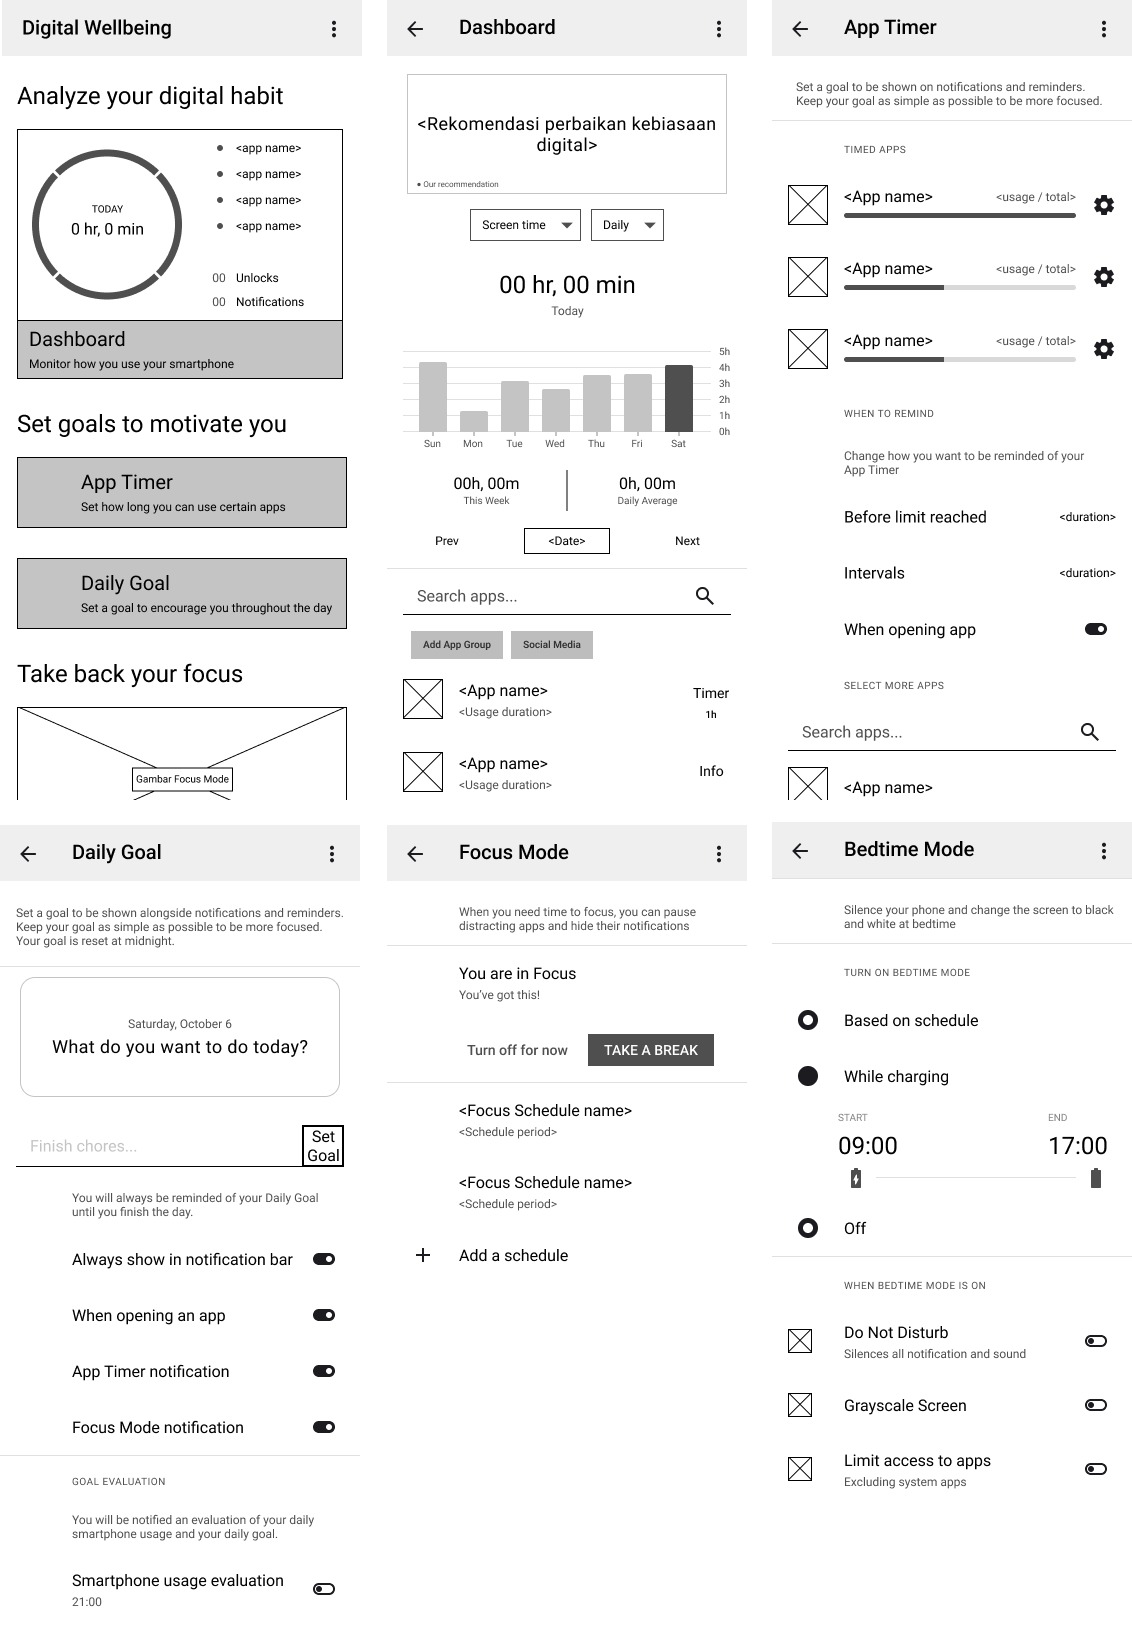
\includegraphics[width=0.9\linewidth]{lofi.png}}
  \caption{Low-fidelity Prototype} \label{fig:lofi}
\end{figure}

\subsection{High-fidelity Prototype}
A high-fidelity prototype implements the design solution as similar as possible to the final product. It contains visual elements dan more complete interaction to accompany the base functionalities. The high-fidelity prototype utilizes the same color pallete from the original Digital Wellbeing app with the main color being green, as well as the same typeface which is Roboto. The interfaces of the high-fidelity prototype can be seen in Fig \ref{fig:hifi}.

\begin{figure}[htbp]
  \centerline{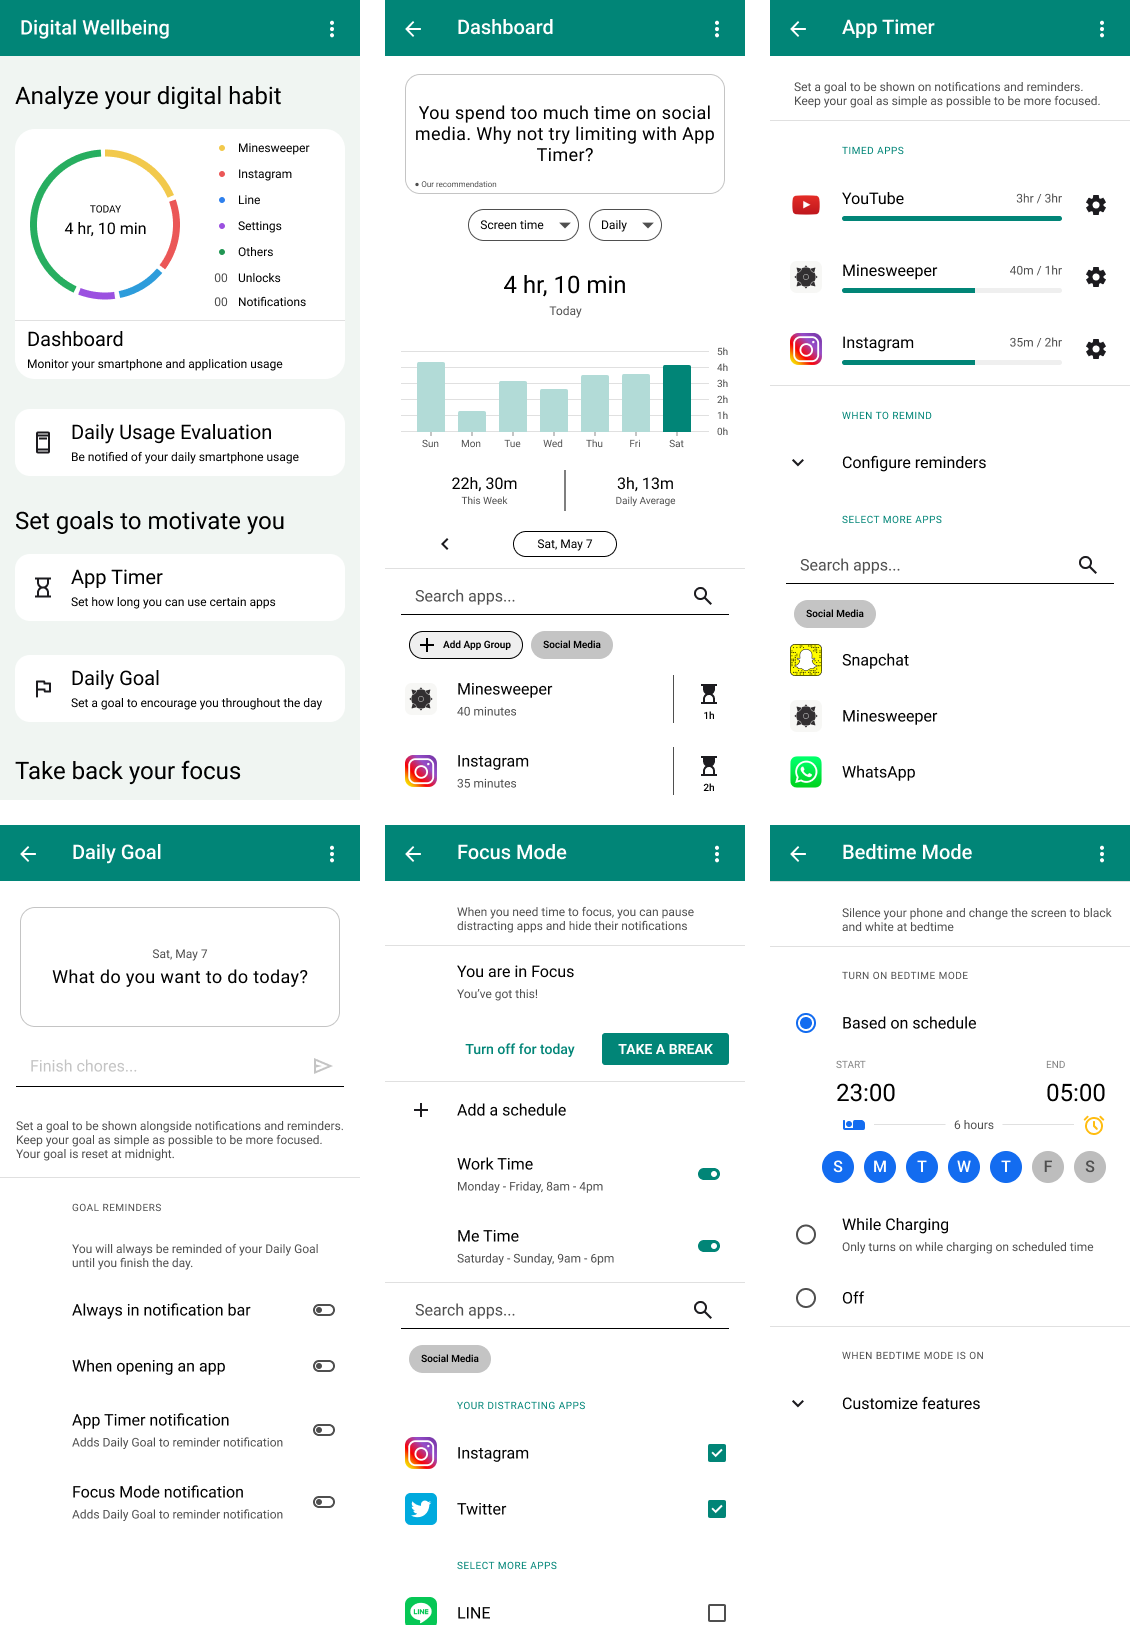
\includegraphics[width=0.9\linewidth]{hifi.png}}
  \caption{Low-fidelity Prototype} \label{fig:hifi}
\end{figure}


\section{Design Evaluation}

Evaluation for the prototypes are done for each iteration based on the User-Centered Design approach. The tests are carried out by 5 participants who belong to the chosen persona. Tests for each iteraton of high-fidelity are done to measure the prototype's achievement of the prioritized usability goals and user experience goals. Table \ref{tab:testing_metrics} explains the mapping of research objectives and testing metrics to each goal.

\RaggedLeft
\begin{table}[htbp]
  \caption{Approaches in Interaction Design \cite{saffer2010designing}}
  \begin{footnotesize}
    \begin{center}
      \begin{tabular}{|m{0.14\linewidth}|m{0.48\linewidth}|m{0.22\linewidth}|}
        \hline
      \textbf{Goals} & \textbf{Testing Objectives} & \textbf{Testing Metrics} \\ \hline
      Overall Usability & Measuring the perceived usability of the high-fidelity prototype & System Usability Scale \\ \hline
      Usability Goal: Utility & Measuring whether the high-fidelity prototype has enough features to meet the user's goals & Specific questions of the System Usability Scale \\ \hline
      Usability Goal: Learnability & Measuring the ease for users to learn and use features of the high-fidelity prototype & Single Ease Question \\ \hline
      User Experience Goal: Helpful & Measuring whether users feel helped in doing their activities by the features provided by the high-fidelity prototype & Intrinsic Motivation Inventory for Value/Usefulness subscale \\ \hline
      User Experience Goal: Motivating & Measuring whether users feel motivated to focus on their work by the features provided by the high-fidelity prototype & Intrinsic Motivation Inventory for Interest/Enjoyment \& Pressure/Tension subscale \\ \hline
    \end{tabular}
    \label{tab:testing_metrics}
  \end{center}
\end{footnotesize}
\end{table}
\justifying

The test results show that the high-fidelity prototipe has Excellent usability, given that all participants gave an SUS score above the 68 point threshold for average usability, with the lowest score being 85.

For measuring the usability goal utility, all participants agree that the various functions in this prototype were well integrated, they disagree that there was too much inconsistency in the prototype, and they also disagree that the prototype very cumbersome to use. This shows that the prototype has met the goal of having good utility.

For measuring the usability goal learnability, the prototype received an average SEQ score of 6.88 from participants. This means that the prototype is easy to learn and has met the usability goal. 

For measuring the user experience goal helpful, all participants gave IMI Value/Usefulness scores above the threshold of 6, with the lowest score being 6.43. This shows that the prototype has met the goal of being helpful.

For measuring the user experience goal motivating, 60\% of participants gave IMI Interest/Enjoyment scores above the threshold of 6, and 80\% of participants gave IMI Pressure/Tension scores below the threshold of 2. These scores show that the prototype has met the goal of being motivating.

\section{Conclusion and Future Works}

After 3 iterations of design and usability testing, it can be concluded that the design solutions have met the user requirements, with prioritized usability goals of utility and learnability, and user experience goals of helpful and motivating. The User-Centered Design process is implemented well involving users in every step of the design process. The design consists of featured features to better reach the goals, which is Search bar, App Group, Activation Schedule, and Daily Goal. The usability goals are met according to SUS and SEQ scores, user experience goals according to IMI scores. 
 
The suggestions for future works related to the topics in this paper are as follows:
\begin{enumerate}
  \item User research can be improved by distributing a survey to people belonging to the target user.
  \item Usability testing of the prototype should include more participants to better measure how the prototype achieves the usability goals and user experiences, with the recommended participants being more than 30 people \cite{nielsengrouptesting}.
\end{enumerate}

\bibliographystyle{IEEEtran}
\bibliography{IEEEabrv,IEEE}

\vspace{12pt}

\end{document}
